Since the electron triggers are not provdied by the $\Pe/\gamma$ physics object group, the trigger efficiencies and the scaling factors are studied using a count tag-and-probe method in this analysis.
\section{Event and sample selection}\label{appendix_sample}
The tag-and-probe electron objects have very similar selections, except that the tag object required to meet the corresponding trigger criteria and tighter selection criteria.

Tag electrons are required to have $\PT < 30/38/35 \GeV$ for different data-taking duration and $|\eta|<2.5 \notin [1.4442, 1.5660]$, and pass the cut based ID at tight working point.

Probe electrons are required to have $\PT > 8 \GeV$ and $|\eta|<2.5$, and pass the cut based ID at tight working point.

Events with exactly two electrons and with at least one electron passing the tag selection criteria and the other electron at least passing the probe selection criteria are chosen.
The tag electron is determined at random if both electrons pass the tag selection criteria.
The required electron pairs must be within $60-120 \GeV$ window as the resonance of the \PZ boson.
The SingleElectron data stream with the pileup reweighting is used since there is only one electron trigger firing in the event.

\section{Results of tag and probe}
A comparison of the trigger efficiency in both data and the simulated sample as a function of probe electron \PT and $\eta$ are shown in Fig.~\ref{fig:appendix_pteff} and~\ref{fig:appendix_etaeff}.
The turn-on curve can be seen in the \PT region due to  the difference in online trigger object reconstruction and offline object reconstruction.

\begin{figure}\centering
    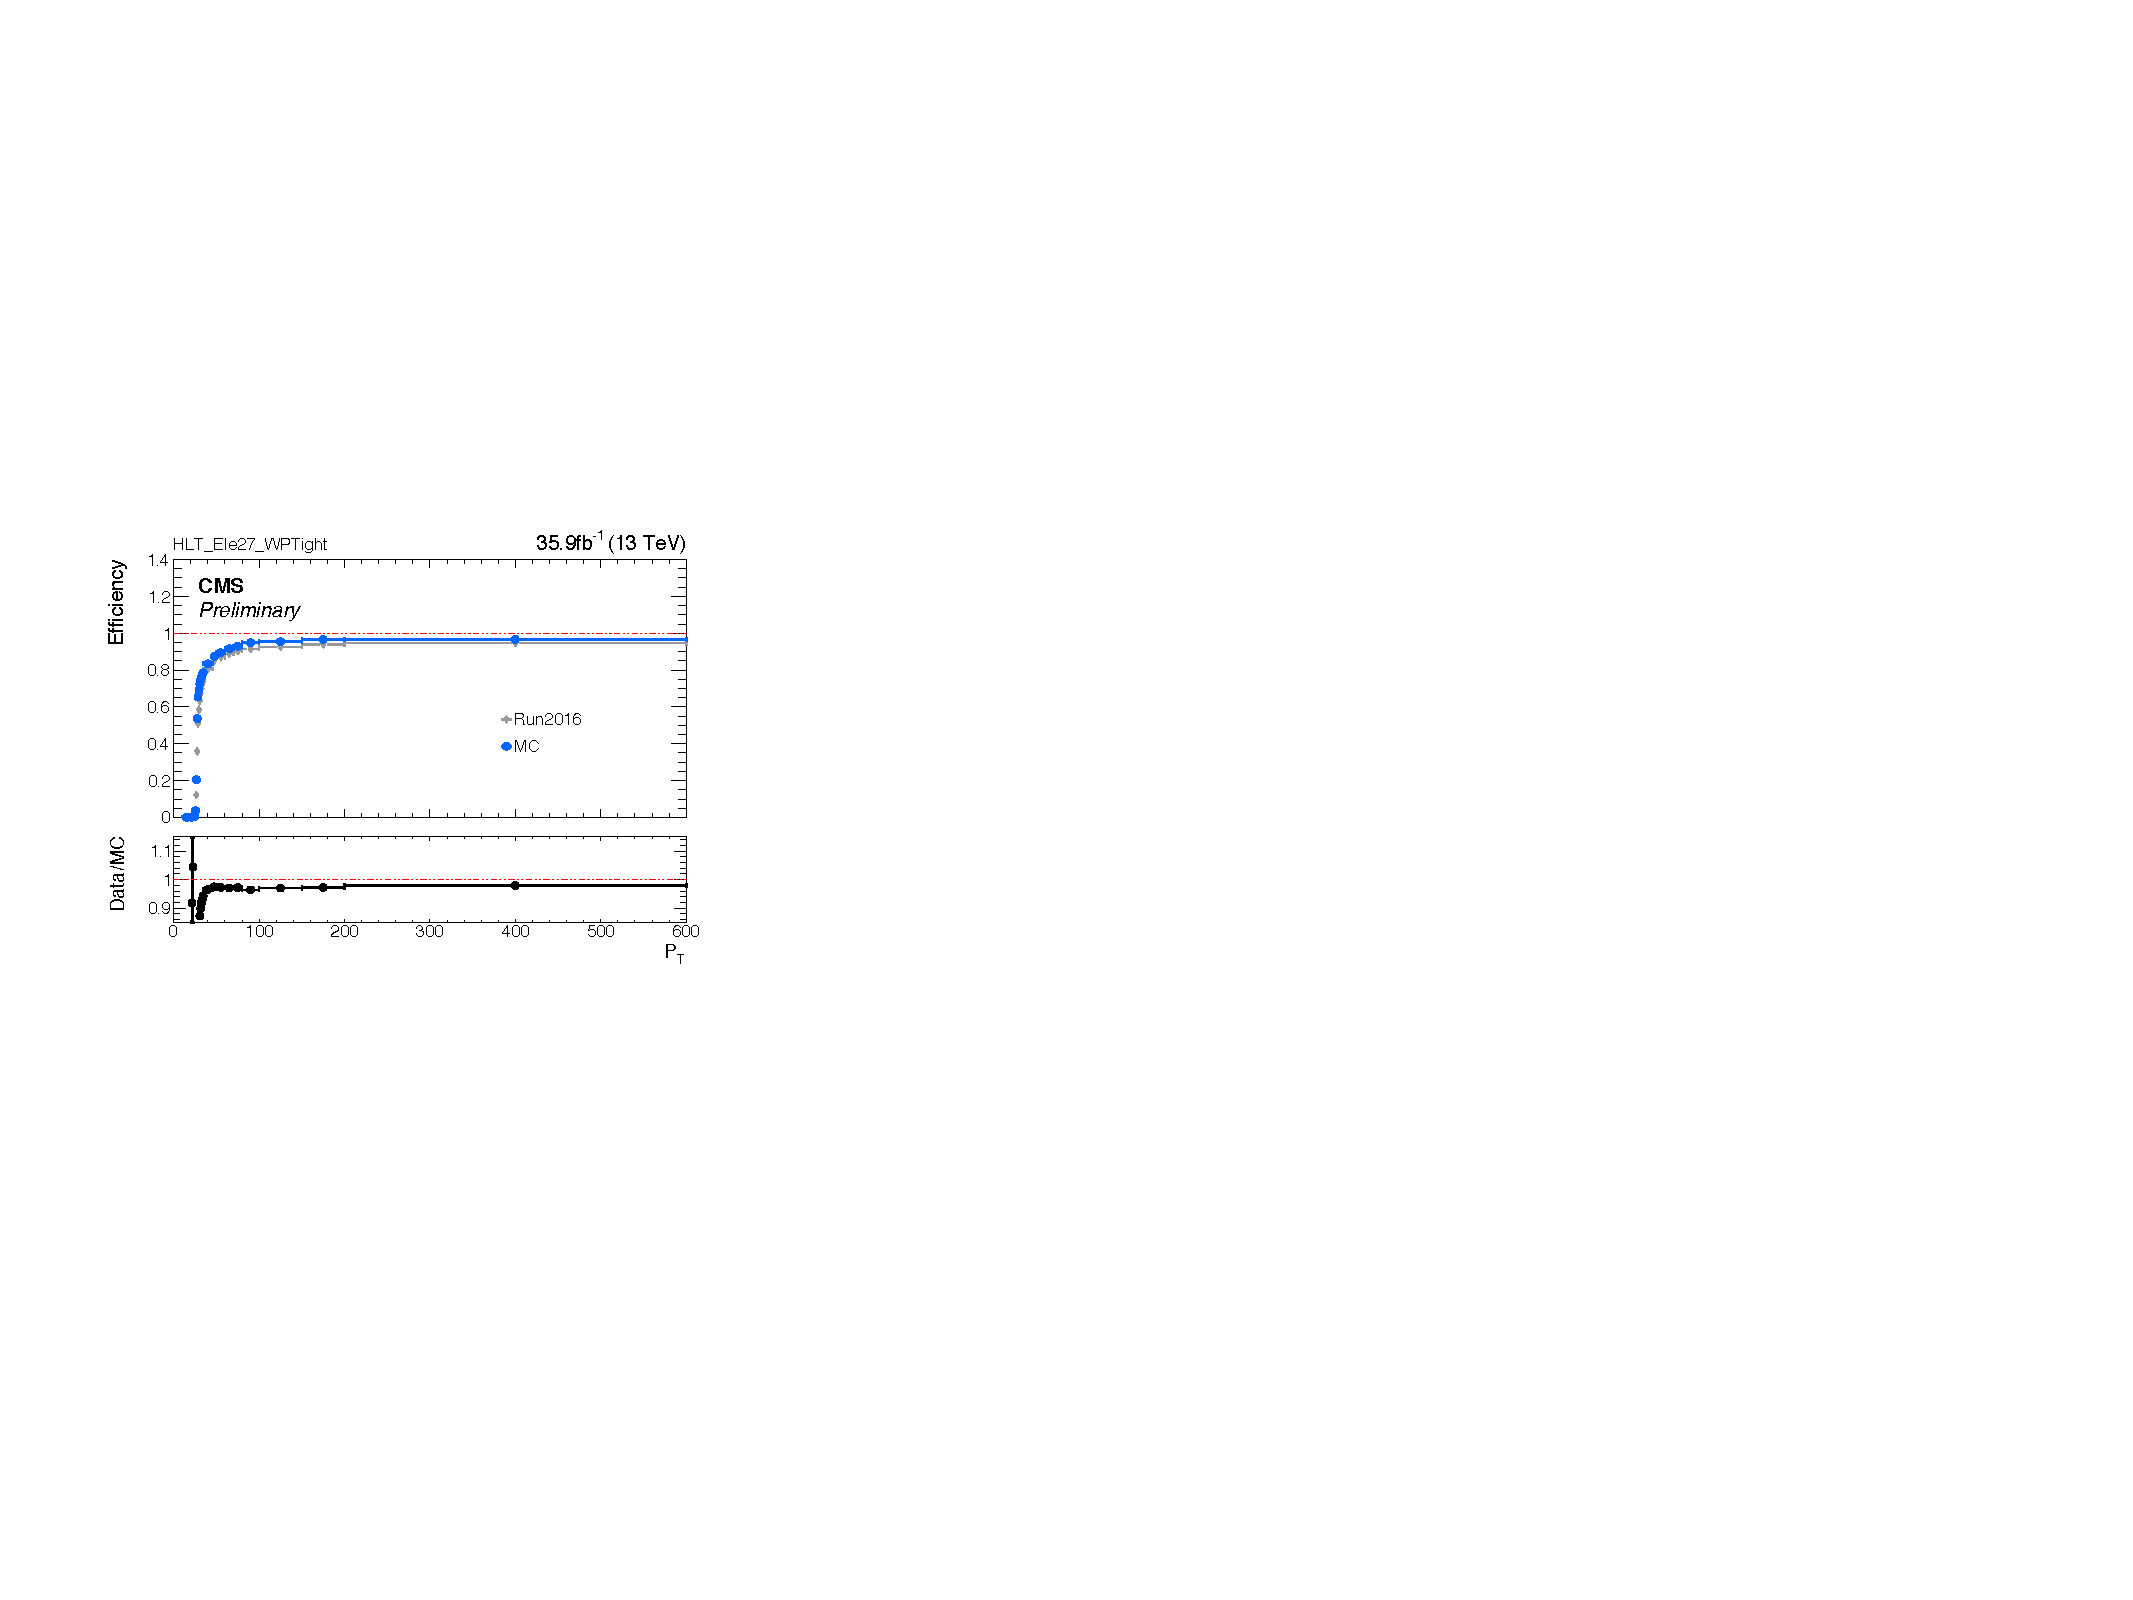
\includegraphics[width=0.7\textwidth]{figure/appendix_16pt.pdf}
    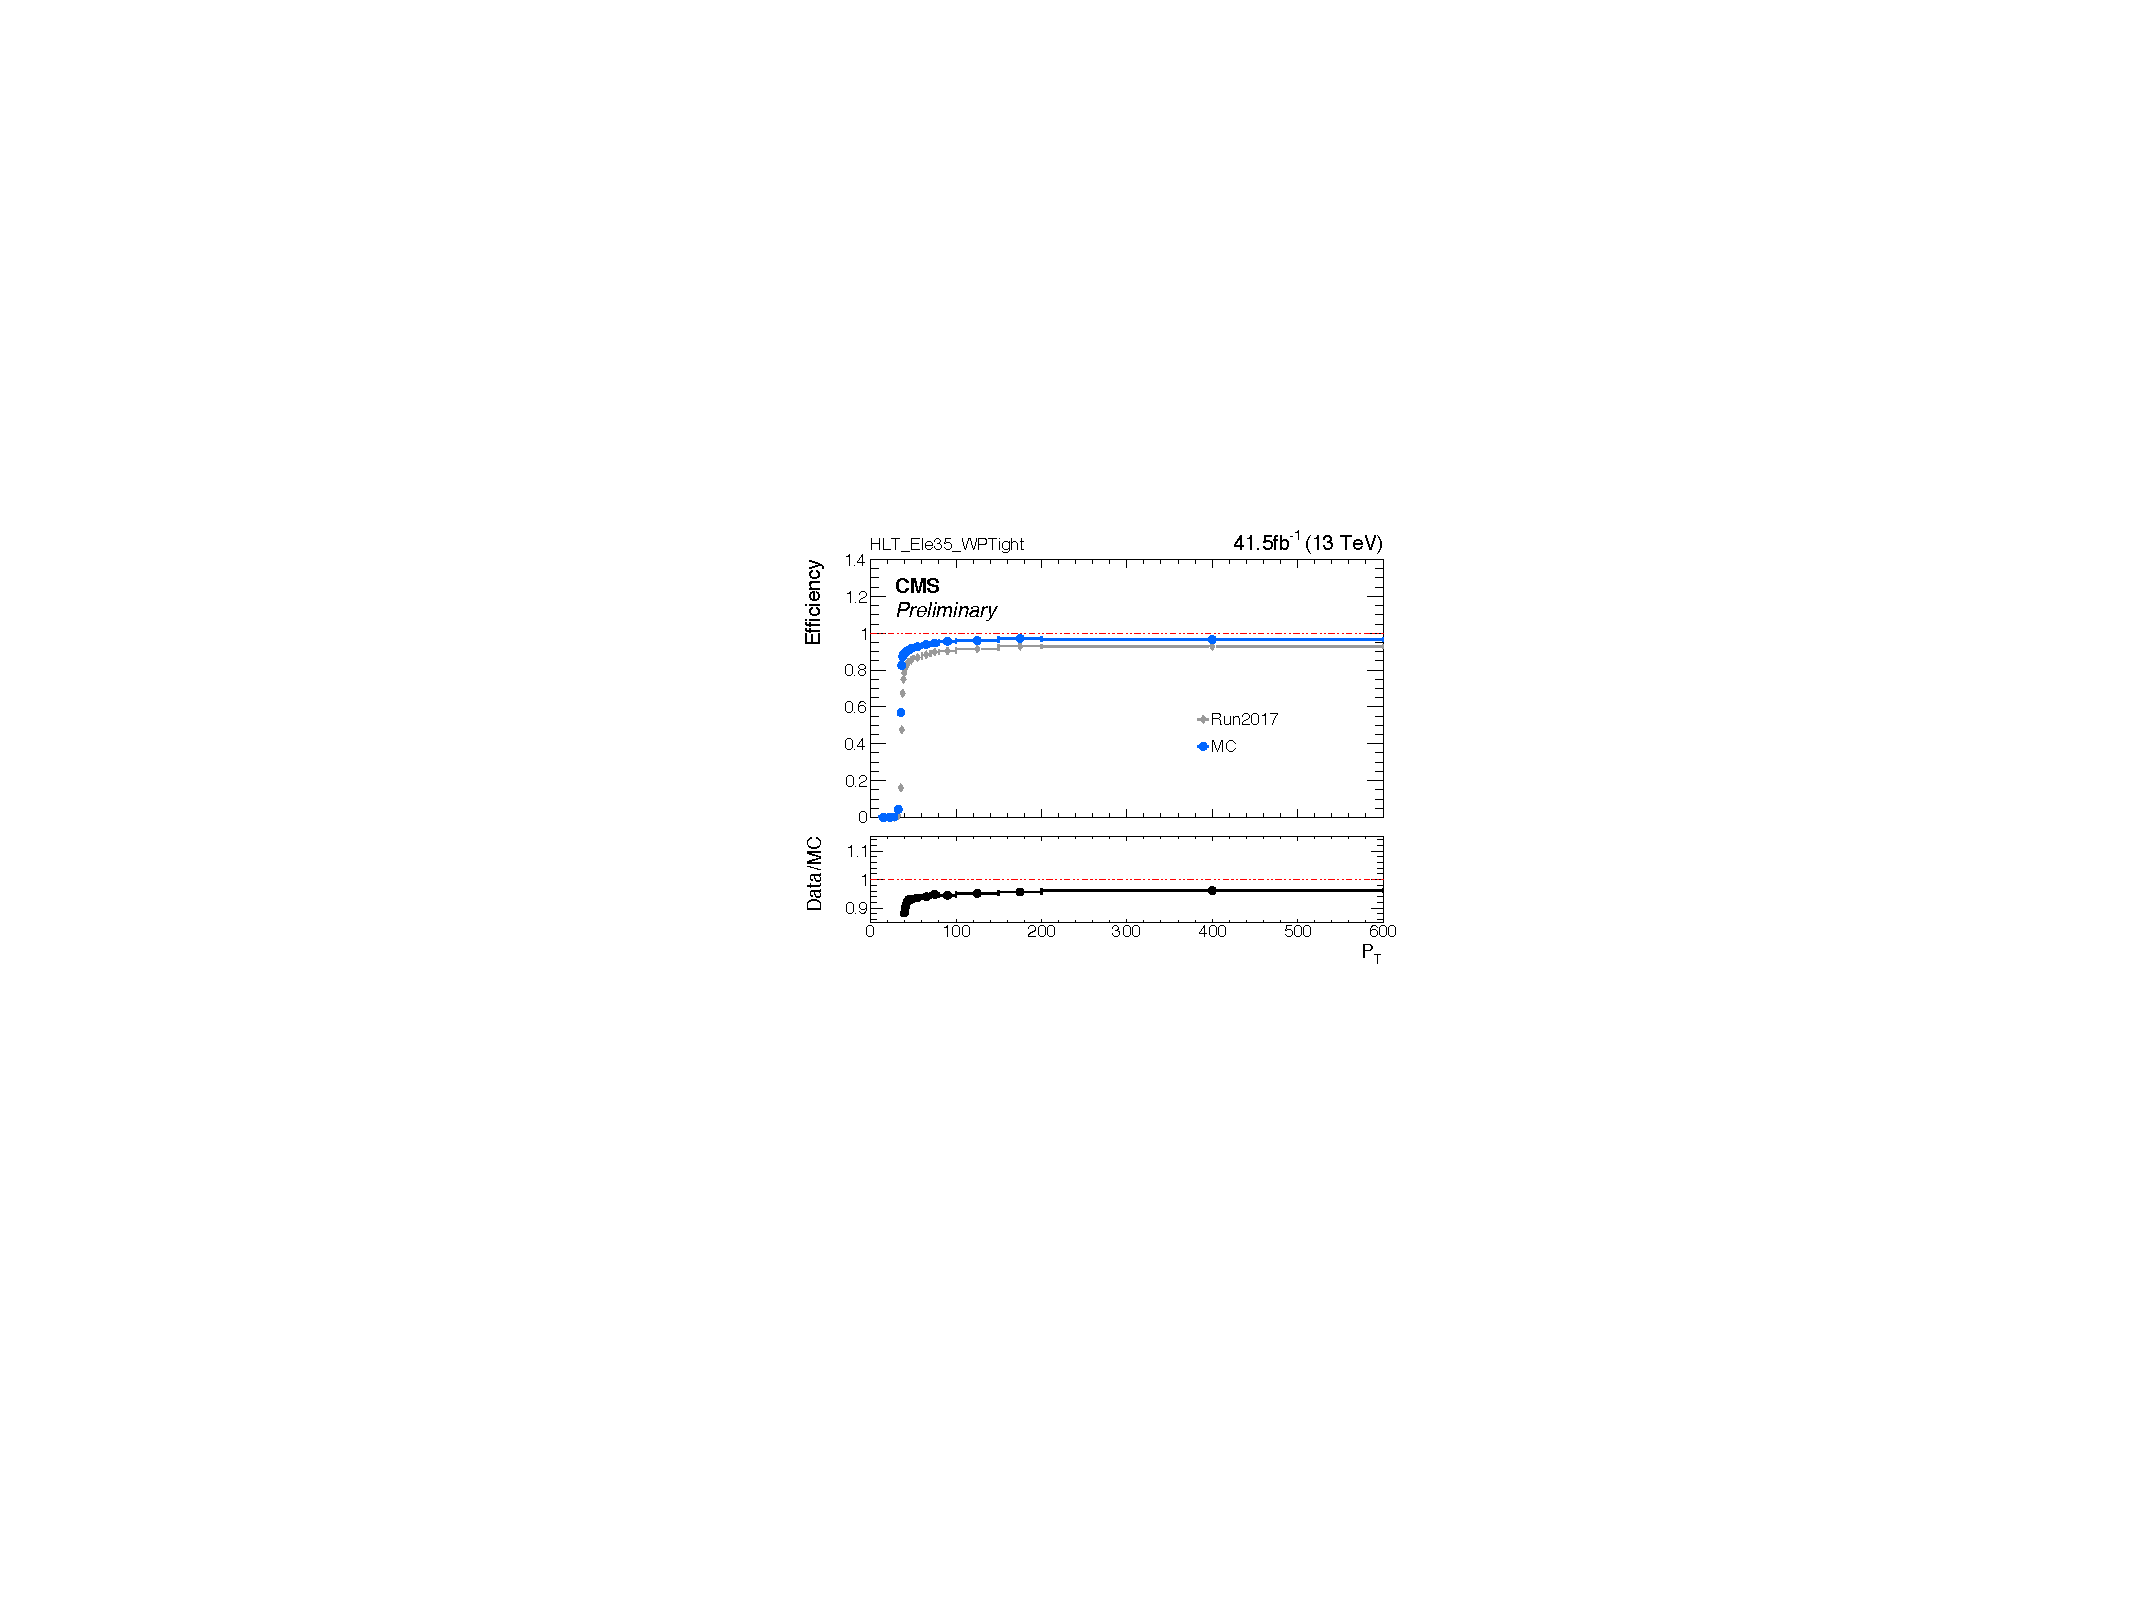
\includegraphics[width=0.7\textwidth]{figure/appendix_17pt.pdf}
    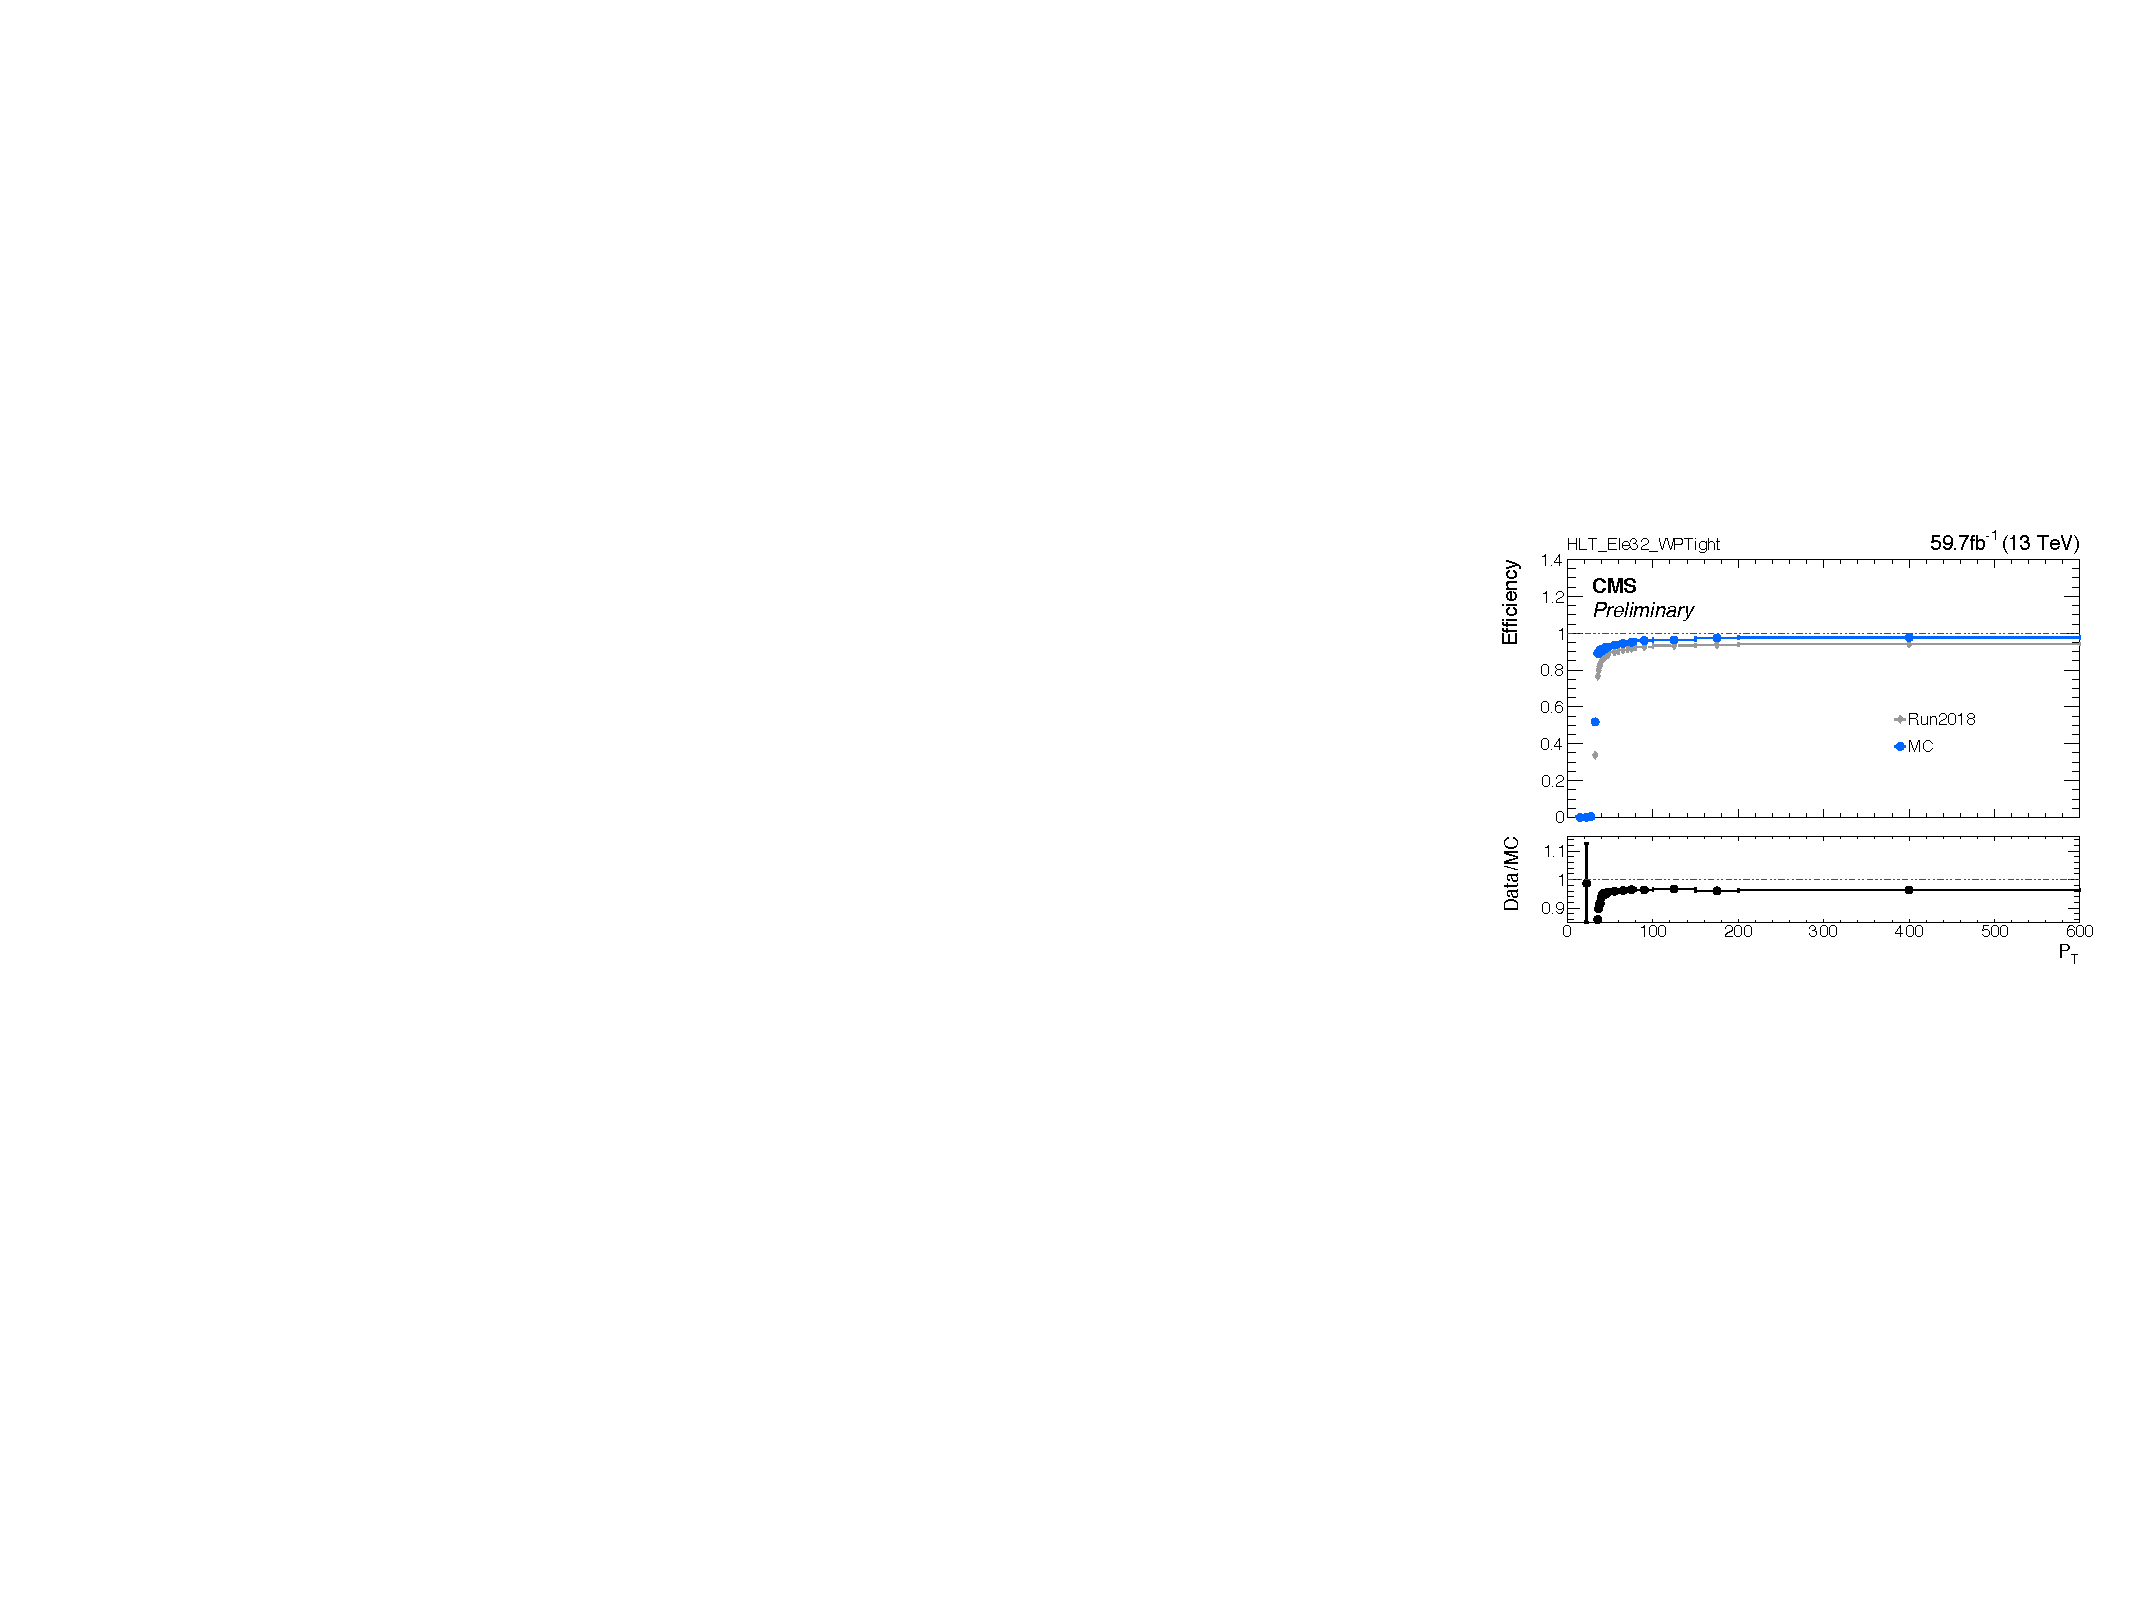
\includegraphics[width=0.7\textwidth]{figure/appendix_18pt.pdf}
    \caption[Trigger efficiency binned by \PT]
    {
        Trigger efficiency binned by \PT with additional kinematic cut of $|\eta|<2.5$ on the probe electron.
        The bottom pad is the scale factor of a particular bin defined as the ratio of trigger efficiency of the data and simulated samples.
    }
    \label{fig:appendix_pteff}
\end{figure}

\begin{figure}\centering
    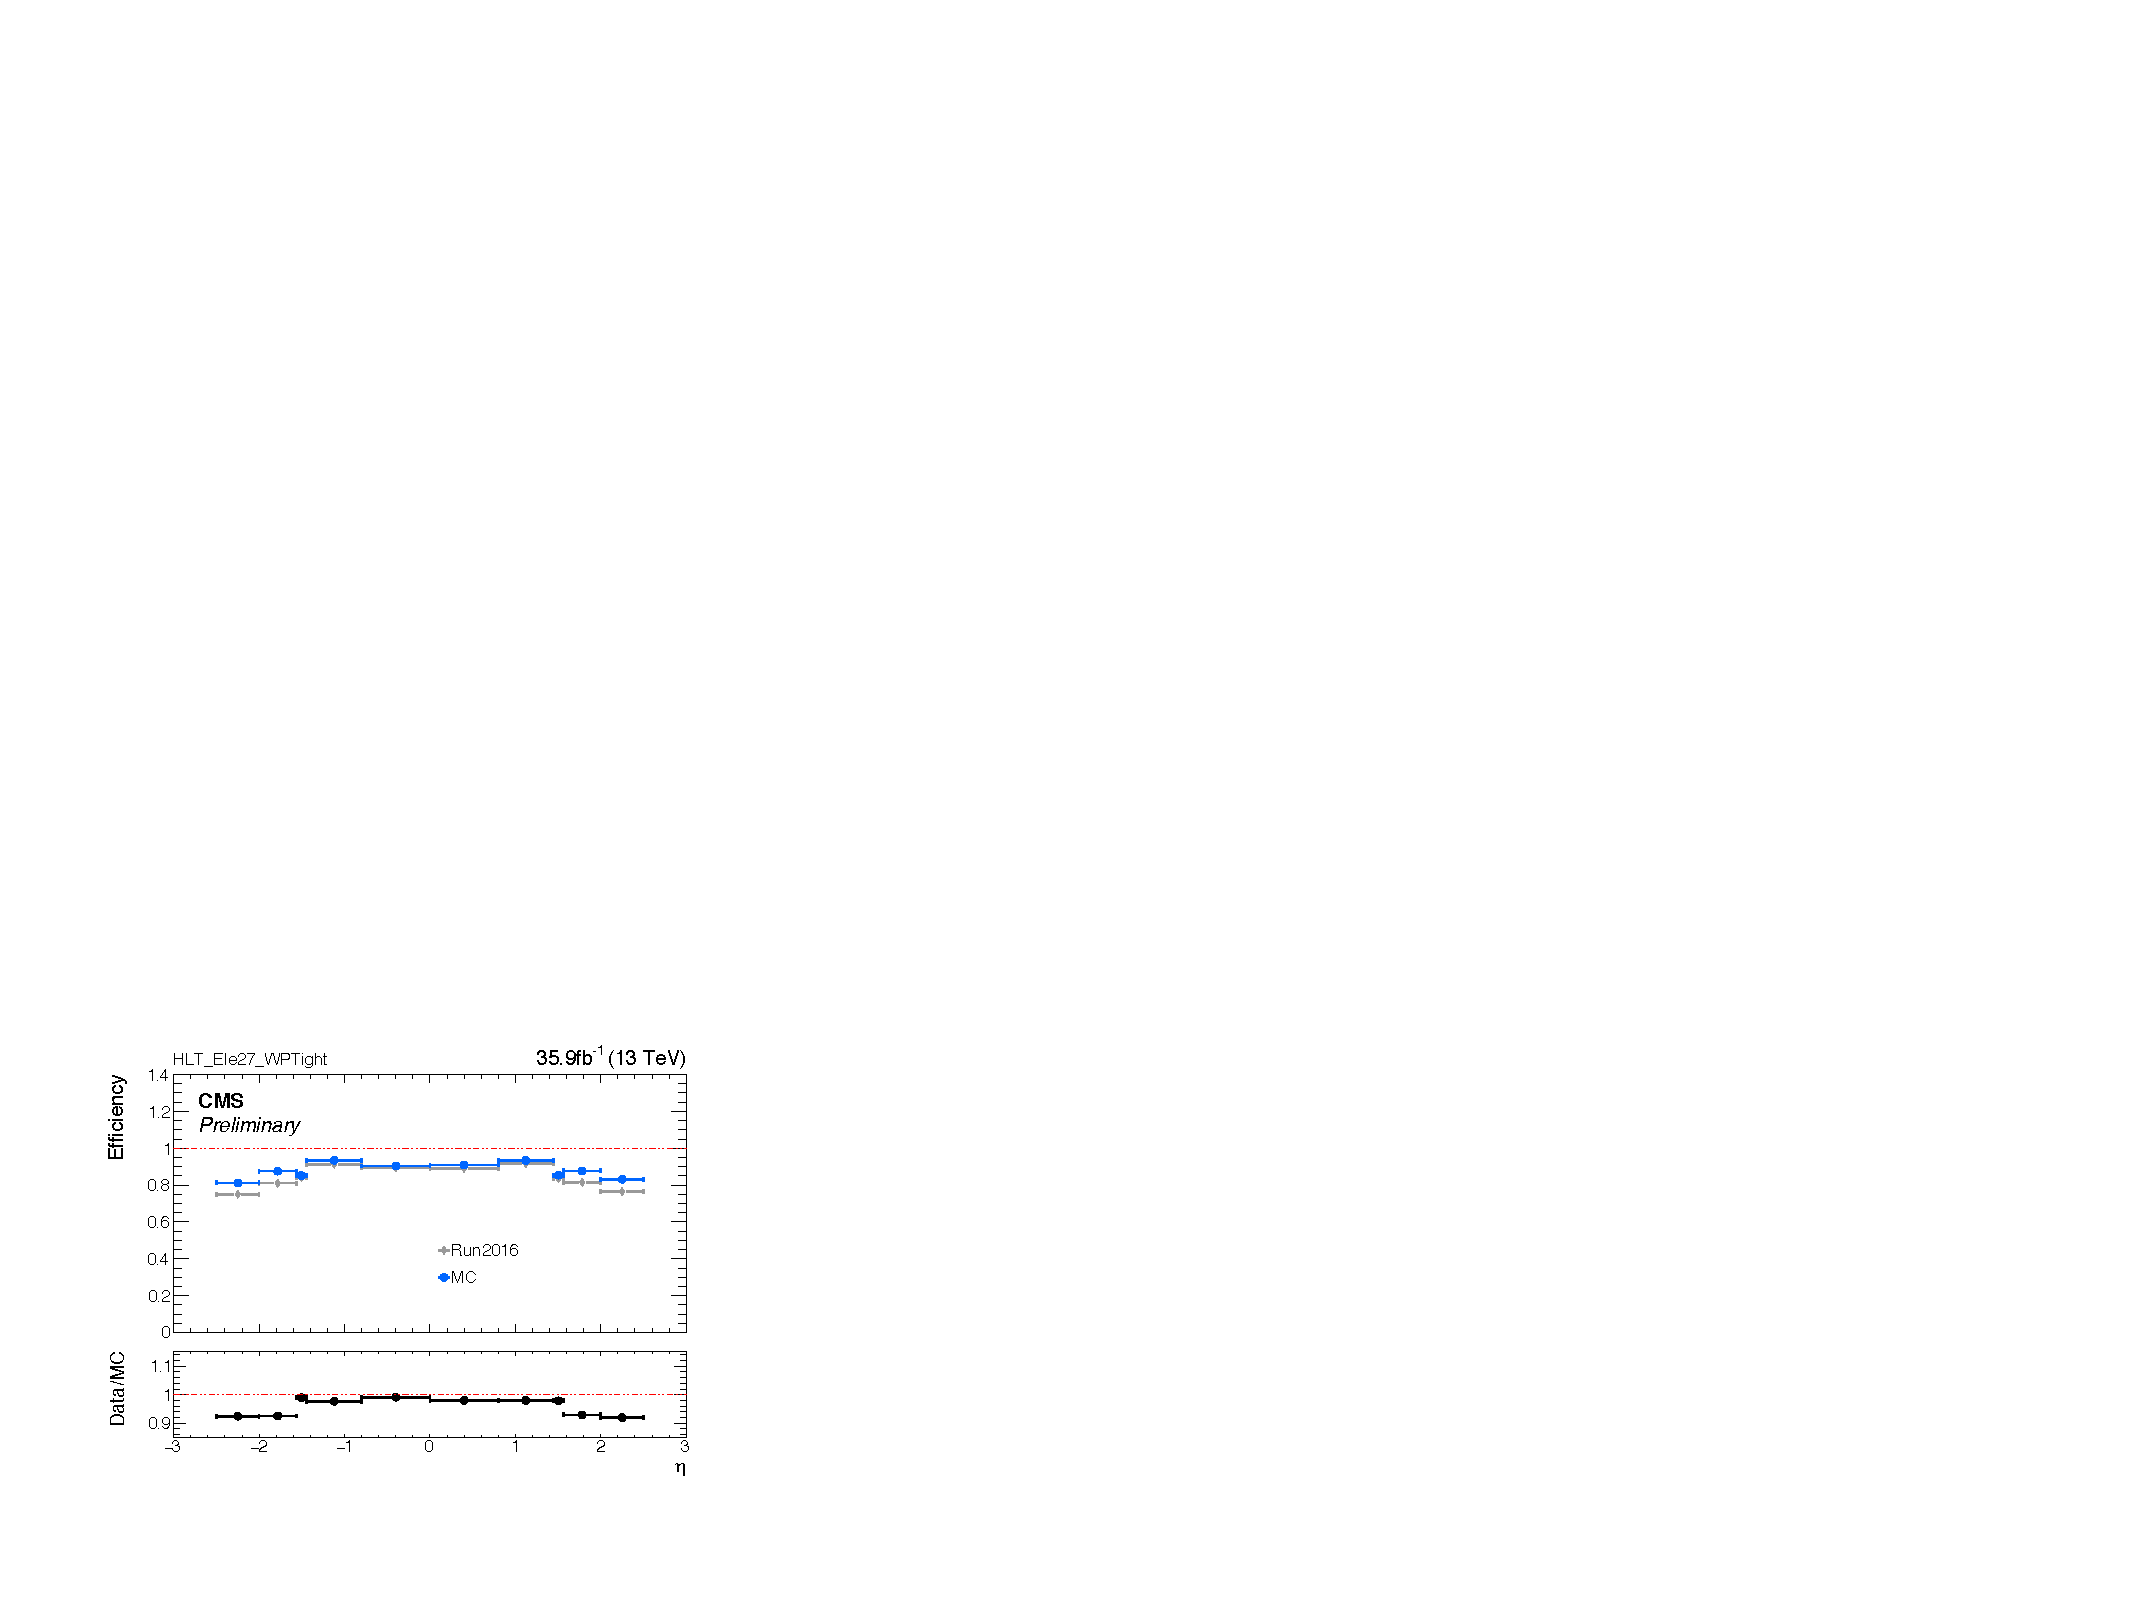
\includegraphics[width=0.7\textwidth]{figure/appendix_16eta.pdf}
    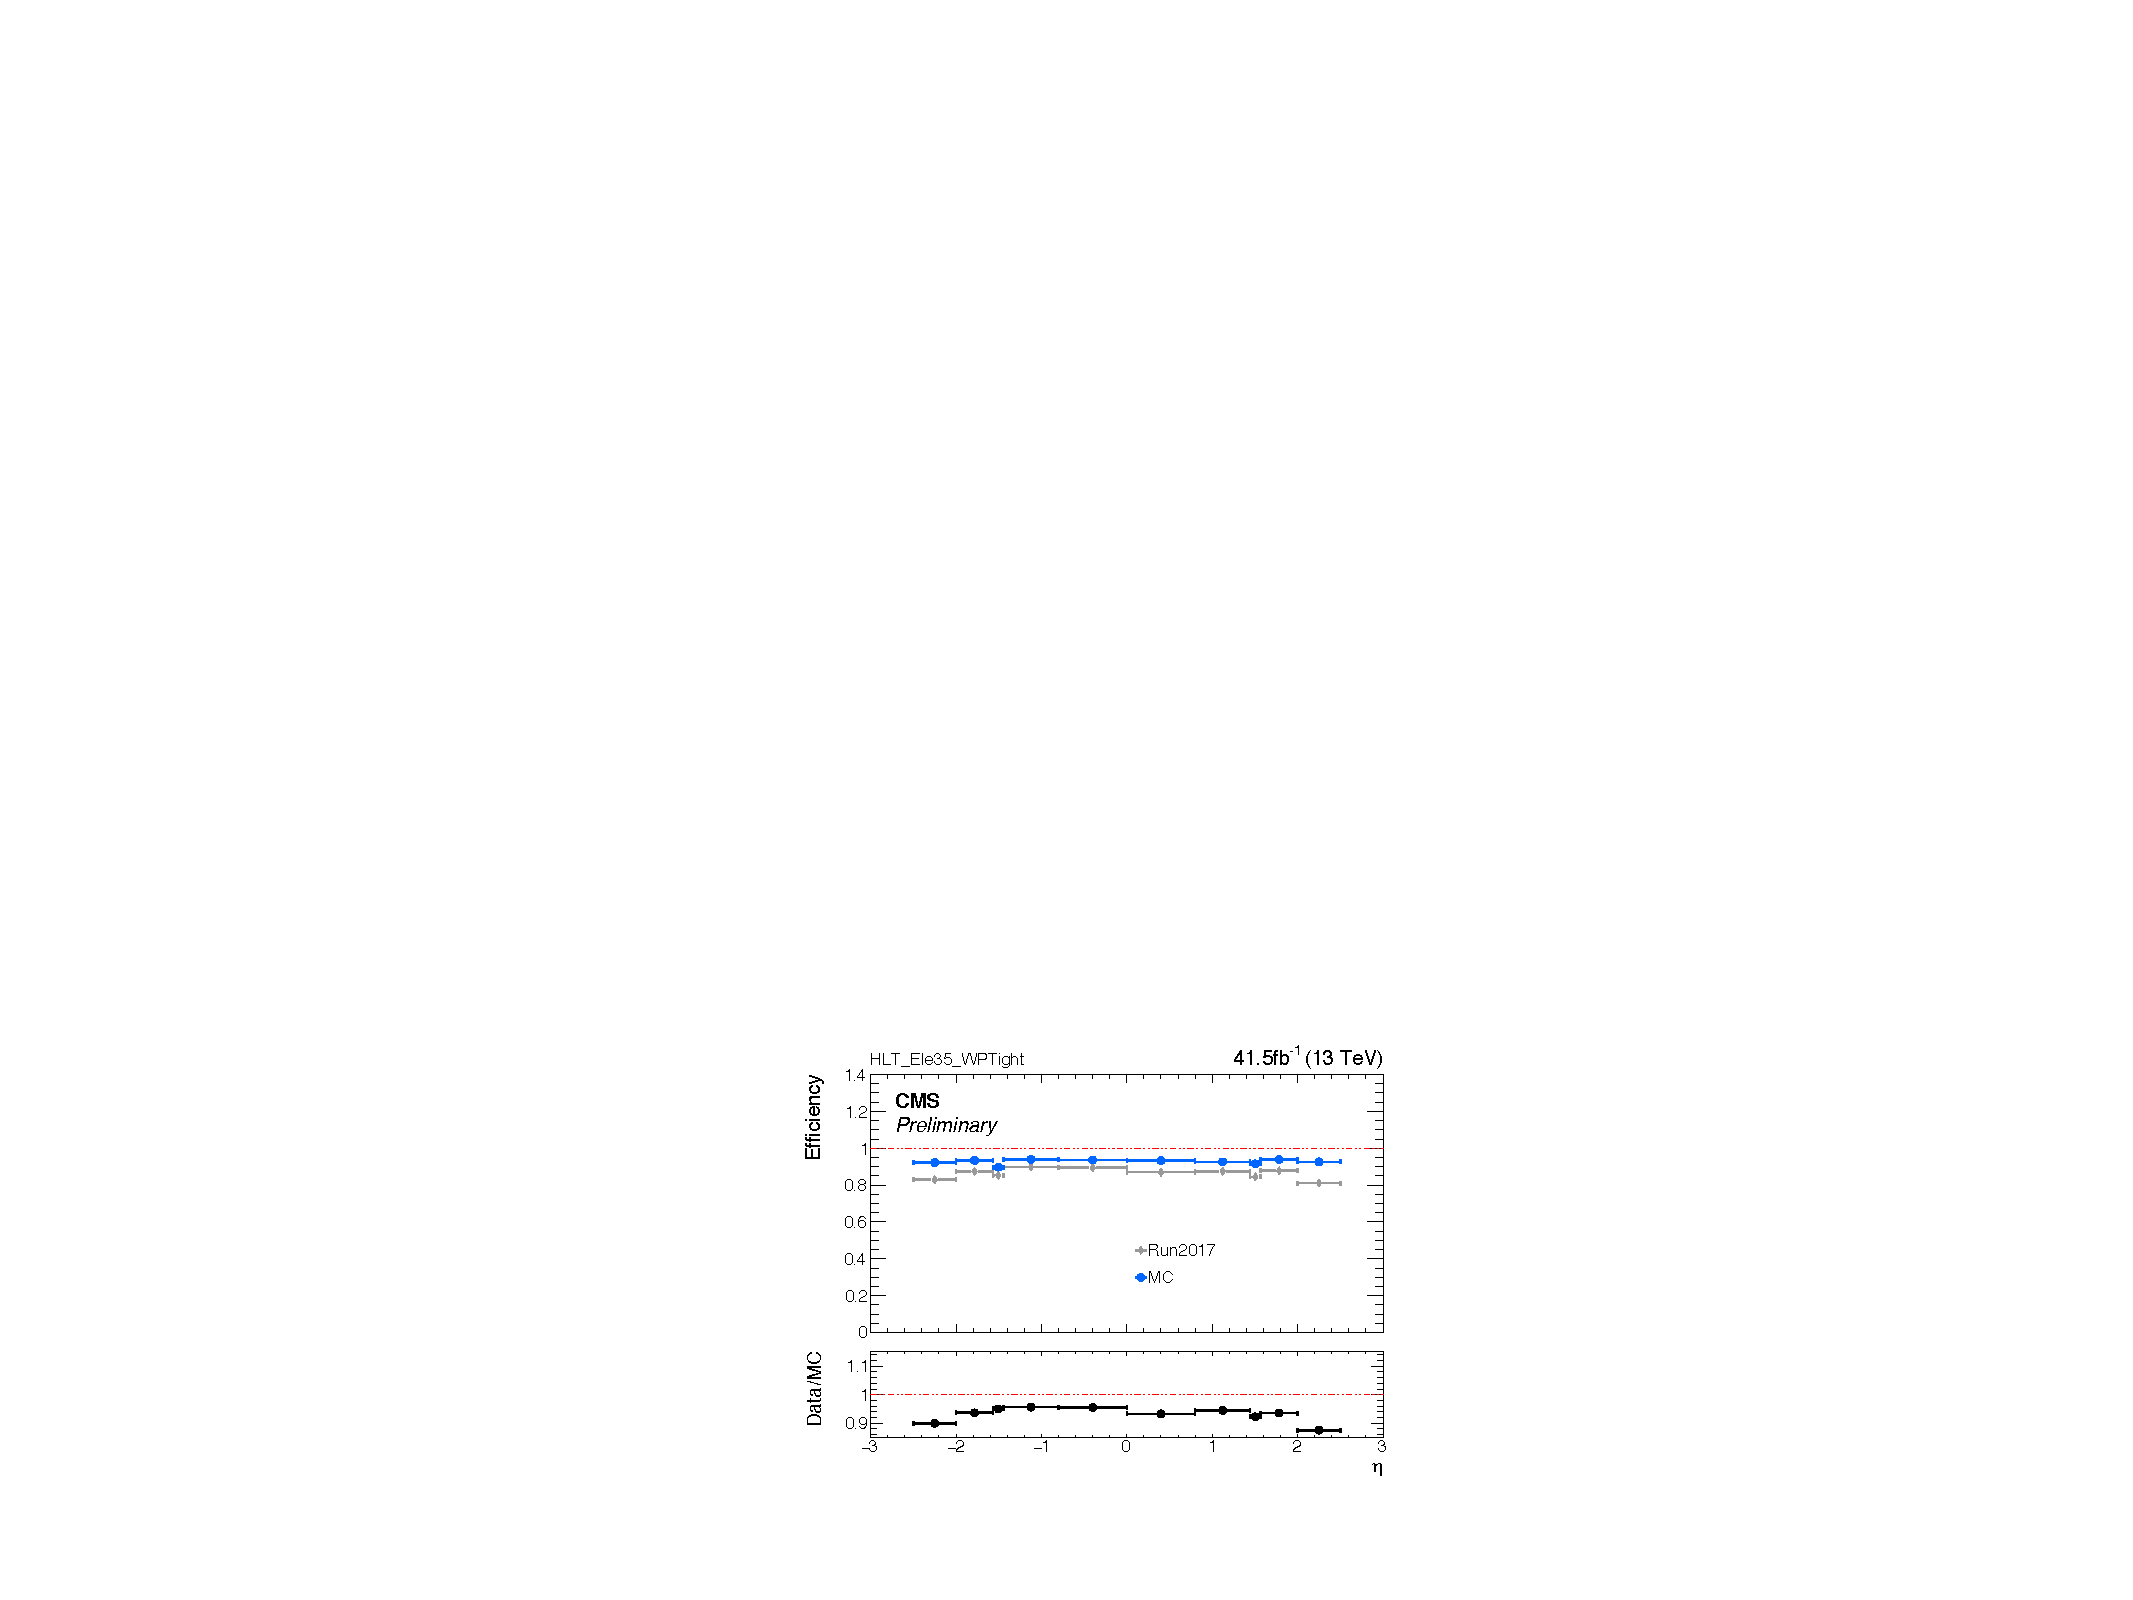
\includegraphics[width=0.7\textwidth]{figure/appendix_17eta.pdf}
    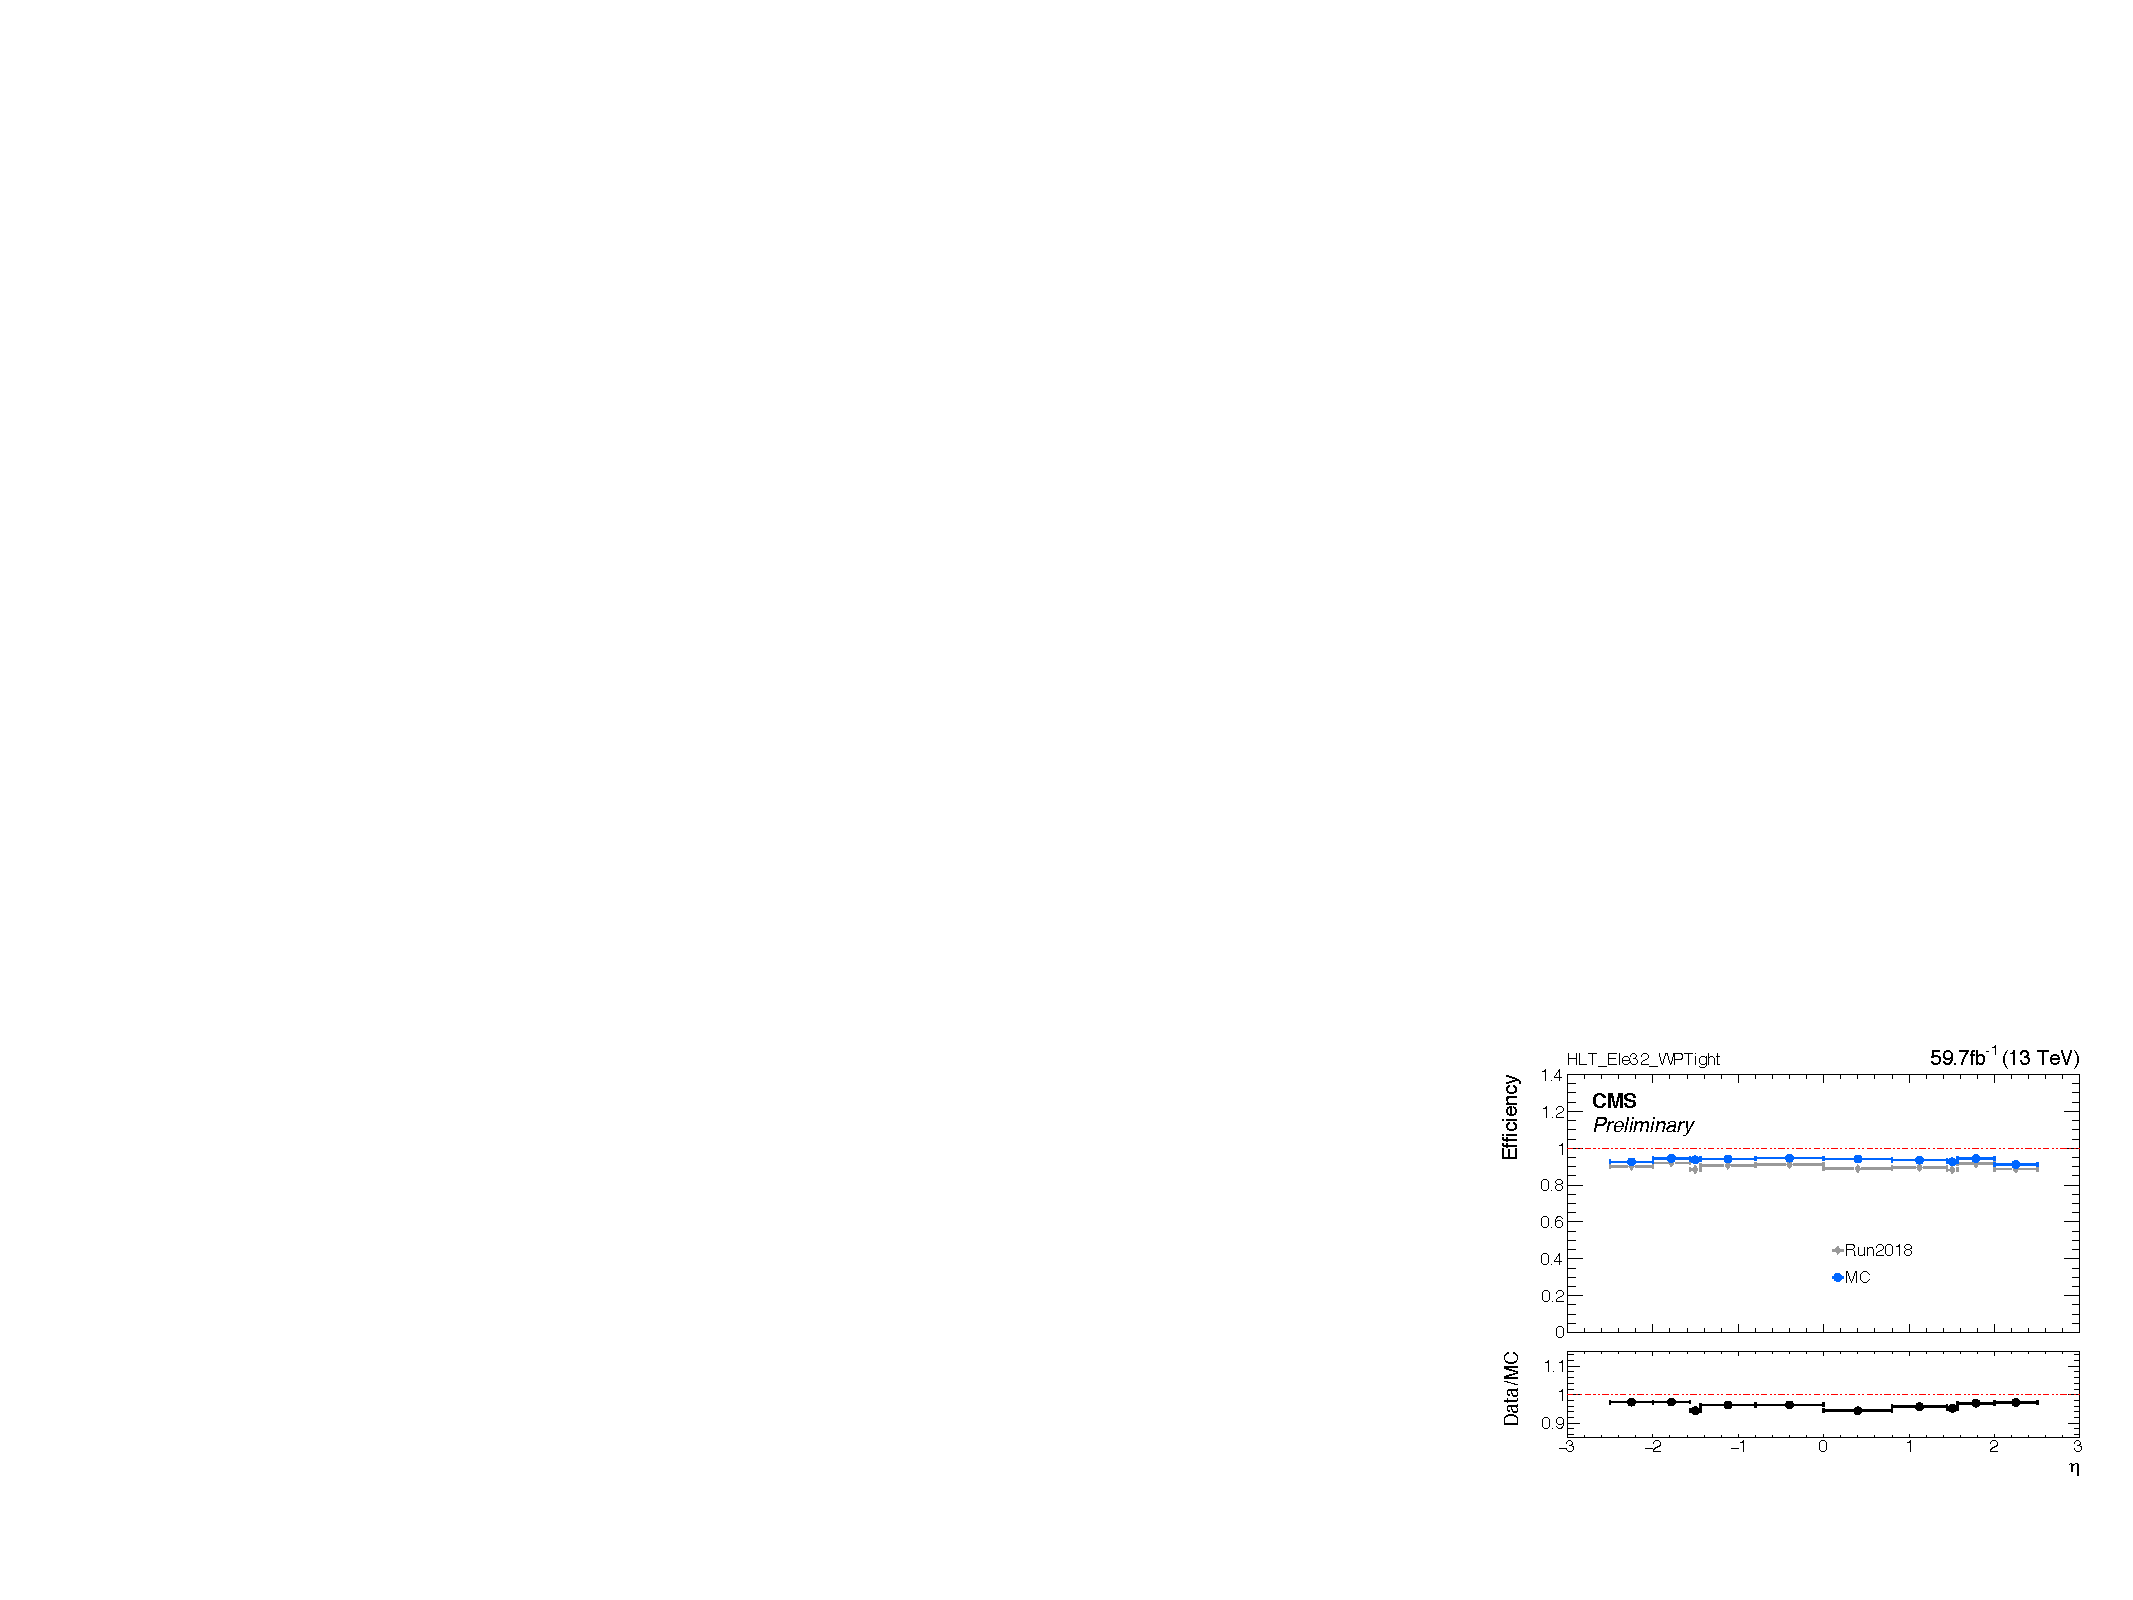
\includegraphics[width=0.7\textwidth]{figure/appendix_18eta.pdf}
    \caption[Trigger efficiency binned by $\eta$]
    {
        Trigger efficiency binned by $\eta$ with additional kinematic cut of $\PT>50\GeV$ on the probe electron.
        The bottom pad is the scale factor of a particular bin defined as the ratio of trigger efficiency of the data and simulated samples.
    }
    \label{fig:appendix_etaeff}
\end{figure}

\section{Systematic uncertainty}
The systematic uncertainties of the tag-and-probe methods are estimated as: 
\begin{itemize}
    \item Raise tag \PT threshold by 5 \GeV.
    \item Shrink the \PZ mass window smaller to $[70-110] \GeV$.
    \item Replace the MC dataset with different generator.
\end{itemize}
The selection and samples in~\ref{appendix_sample} are used as the central value of the trigger scale factors, and the difference in scale factors obtained with different selection and samplers will be used as the systematic uncertainty.
The differences are consistently smaller than $1\%$ and thus a $1\%$ systematic uncertainty for all bins is placed on top of the statistical uncertainties.
